\begin{center}
	\vspace{1em}
    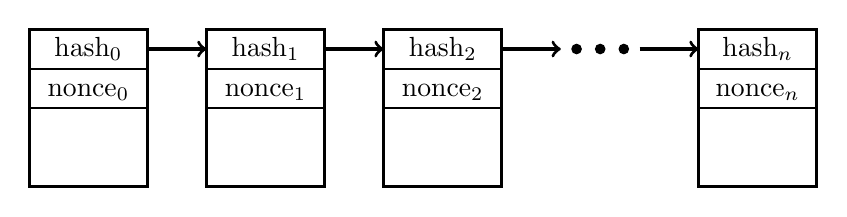
\begin{tikzpicture}
    % blockchain figure

    % boxes (w,l) = (1.5,2)
    \draw [very thick] (0,0) rectangle (1.5,2);
    \node at (0.75,1.75) {hash$_0$};
    \draw [thick] (0,1.5) -- (1.5,1.5);
    \node at (0.75,1.2) {nonce$_0$};
    \draw [thick] (0,1) -- (1.5,1);

    \draw [very thick] (2.25,0) rectangle (3.75,2);
    \node at (3,1.75) {hash$_1$};
    \draw [thick] (2.25,1.5) -- (3.75,1.5);
    \node at (3,1.2) {nonce$_1$};
    \draw [thick] (2.25,1) -- (3.75,1);

    \draw [very thick] (4.5,0) rectangle (6,2);
    \node at (5.25,1.75) {hash$_2$};
    \draw [thick] (4.5,1.5) -- (6,1.5);
    \node at (5.25,1.2) {nonce$_2$};
    \draw [thick] (4.5,1) -- (6,1);

    \draw [very thick] (8.5,0) rectangle (10,2);
    \node at (9.25,1.75) {hash$_n$};
    \draw [thick] (8.5,1.5) -- (10,1.5);
    \node at (9.25,1.2) {nonce$_n$};
    \draw [thick] (8.5,1) -- (10,1);

    % lines (length 0.75)
    \draw [->, very thick] (1.5,1.75) -- (2.25,1.75);
    \draw [->, very thick] (3.75,1.75) -- (4.5,1.75);
    \draw [->, very thick] (6,1.75) -- (6.75,1.75);
    \draw [->, very thick] (7.75,1.75) -- (8.5,1.75);

    % dots
    \draw [fill=black] (6.95,1.75) circle (0.06);
    \draw [fill=black] (7.25,1.75) circle (0.06);
    \draw [fill=black] (7.55,1.75) circle (0.06);

    \end{tikzpicture}
    \captionof{figure}{Prototypical Proof of Work Blockchain \label{fig:blockchain}}
\end{center}
